%
%  $Author: awl8049 $
%  $Date: 2008/10/01 18:46:40 $
%  $Revision: 1.1 $
%
%\documentclass[times, 10pt,twocolumn]{article} 
\documentclass[12pt,onecolumn]{ULieeetran} 
\usepackage{setspace}
\usepackage{graphicx}
\usepackage{authblk}
\usepackage{amsmath}
\usepackage{amsthm}
%\usepackage{pdfsync}
\pagestyle{plain}
\begin{document}
\title{Alleviating Adverse Thermal Impacts of Cache Affinity in
  Multi-Core Processors}
\author[]{~} 
\affil[]{~}
% \author[*]{Adam Lewis} 
% \author[*]{Soumik Ghosh} 
% \author[*]{N.-F. Tzeng}
% \affil[*]{Center for Advanced Computer Studies\\ 
%  University of Louisiana\\ 
%  Lafayette, Louisiana 70504\\ 
%  \{awlewis,sxg5317,tzeng\}@cacs.louisiana.edu
% }
\maketitle
\newtheorem{defn}{Definition}
\newtheorem{thm}{Theorem}
\thispagestyle{empty}
\doublespacing
\begin{abstract}
  While scheduling threads on the same processors repeatedly enjoys high
  performance due to cache affinity (i.e., reuse), a scheduler may also
  rely on process migration among the cores of a multi-core processor to
  manage energy consumption and regulate thermal impacts, in addition to
  further performance improvement.  This work introduces a simple
  full-system power model to accurately predict system power consumption
  (to within a four percent error) and to estimate system and processor
  die temperatures for an objective function useful for the thread
  scheduling process.  The introduced full-system power model determines
  when to apply our measurement-based power management techniques on a
  working system; making use of collected hardware and software metrics
  (such as cache and bus behavior counters, per-core die and ambient
  temperature readings, etc.).  The objective function enables the
  operating system scheduler to decide the best set of thread
  assignments to minimize the energy consumed by service requests while
  accounting for thread affinity, energy management, and thread
  performance deadlines. We have employed the SPEC CPU2006 benchmark
  suite to validate the effectiveness of the power model and objective
  function.
\end{abstract}

\section{Introduction}
\label{sec:Introduction}

Thread affinity exists between a thread and a processor (or processing
core) when the processor cache has accumulated some amount of the
process state.  This affinity may be high or low depending upon how much
of the process state exisits in the cache. Modern operating system
schedulers take advantange of high cache affininty to improve
performance by scheduling threads on a recently used processor when
possible so as to reduce cache miss penalty.

At the same time, operating system schedulers use process migration
amongst processing cores as a mechanism to improve performance, manage
energy consumption and control thermal regulation. Frequent migration of
thread state prevents the scheduler from exploiting cache affinity.
Thus, the scheduler must find a balance between these conflicting
requirements in its search for the best assignment of threads to
processing cores.

There are three processor configurations typically found in servers:
single core uniprocessors, multicore uniprocessors, and multicore
multiprocessors~\cite{Kazempour2008}.  The configurations are
distingushed by the number of processor cores and the physical
placement of cores with respect to last-level shared processor cache.
In our study, we consider the most common of server configurations:
multicore multiprocessor.

The performance effects of cache affinity is very well understood for
uni-core processors and is beginning to be understood for mutlicore
processors~\cite{Kazempour2008}.  However, the power and thermal
effects of cache affinity remain a topic of research.  

In this experimental study, we make the following contributions:
\begin{itemize}
\item An experimental study of the impact on power consumption and
  processor die temperature of a collection of HPC-oriented workloads
  from the SPEC CPU2006 benchmark.
\item A linear model of system and processor die temperatures that can
  be used as an objective function in the thread scheduling process in
  an operating system.
\end{itemize}

\section{Background and Prior Work}
\label{sec:prior}

The rising popularity of multicore processors in servers leads to
performance issues that did not exist for single-core symmetric
multiprocessors (SMP) as the operating system can assume in the SMP case
that the CPU is a single dedicated resource.  Thus, the scheduler can
take advantage of this fact and return a previously executed thread onto
the same processor upon which it was running when it was swapped out.
Thus, the process can avoid performance issues by taking advantage of
any state that may remain in cache from before the thread swap
occurred.  This is possible because we treat the resource as a single,
dedicated resource.

In the multicore environment, this assumption no longer holds as the
processor has multiple processing cores that often share a single
last-level cache.  In this case, you have concurrently running threads,
described in~\cite{Fedorova2008} as \textit{co-runners}, sharing this
last-level cache with the allocation of the cache controlled by the
hardware rather than the operating system.   As result, the sharing of
the cache quickly becomes unfair with a resulting increase in cache miss
rates. Fedorova, \textit{et. al.}~\cite{Fedorova2008} introduced the
concept of a \textit{cache-fair algorithm} that addresses unequal cache
allocation by redistributing CPU time to threads to account for the
performance decrease caused by unfair cache sharing.   However, this
algorithm did not take into account that the operating system can
acquire information about cache allocation policy from the hardware.

Power models are used to predict to when to apply power management techniques
to a working system. These models can be classified into two
broad categories: detailed analytical power models and high-level
blackbox models~\cite{Rivoire2008b}. Analytical models use detailed
knowledge of the underlying hardware to either simulate the energy
consumption or directly measure energy comsumption at the hardware
level.  Simulation can provide detailed analysis and breakdown of energy
consumption; however, they are slow and do not scale well to realistic
applications and large data sets.  Simulation-based models do not fit
well into scensarios where dynamic optimization of application
performance is required~\cite{Economou2006}.

Measurement-based models attempt to collate power measurements with
hardware and software performance metrics.  Two distinct classes of
metrics have been used in these models: processor performance counters
and operating system performance metrics.  Processor performance
counters are hardware registers that can be configured to count various
microarchitectural events such as branch mispredictions and cache
misses.  In general, the number of countable events exceed the number of
available registers.  As result, models that use these counters
time-multiplex different sets of events on the available registers.
While this allows for more events to be monitored, it results in
increased overhead and lower accuracy due to sampling
issues~\cite{Economou2006}\cite{Rivoire2008a}.

The question becomes what set of processor performance counters provide
the best insight into both cache performance and energy consumption?
The most popular set of metrics used in previous work has involved
variations on lastlevel miss rates and processor cycles per
instruction~\cite{Tam2007}\cite{Banikazemi2008}.    

\section{Thread Affinity: Negative Thermal Impact?}
\label{sec:affinimpact}

Where are the hotspots on a processor?  Reference prior work.

How does putting stuff back into the same place make the problem worse?
What about shared resource contention?

How do you back up these claims?


\section{System Energy Model}
\label{sec:modelstruct}

Understanding the thermal impacts of affinity requires that we have a
clear understanding of the energy consumption of the processor and the
resulting system thermal map. We start by considering the type of power
supplied into the system.

Most server blades operate on an AC input.  The DC output from the power
supply in our experimental platform is delivered in the domains of
+/-12V, +/-5V, and +/-3.3V \cite{SSI2004}. In the case of the Sun server
used in this study, two 12 Vdc lines supply power to the processor's
hard drive(s) and cooling fans in the system. The 5 Vdc and 3.3 Vdc lines
are dedicated to supplying power to the support chips and peripherals
on the board.  Most switched mode power supplies for servers have a
power conversion efficiency from AC to DC of 72 - 80 \% , depending on
the load of the system. Typically for a server that is idling, i.e. is
running the operating system and no other jobs, the power consumption is
close to 40 - 42\% of the rated power of the system (in our case
450W). The conversion efficiency increases to about 80\% when heavily
loaded , and the SMPS regulates the power supply to work at 75\%
conversion efficiency at loads over 50\% of the rating.

Hence we can see that at the very outset that we lose 20\% of the
power supplied into the system to conversion losses even for the best
conversion factors. Studies have shown \cite{ton2008} that most DC
systems perform better in terms of power efficiency than AC systems. A
typical AC-based server system has a power supply efficiency of 73\% as
compared to a 92\% for a DC system. Also, the overall system efficiency for a
AC system is 61\% as compared to 85\% for a DC system.
\begin{figure}[htbp]
\begin{center}
     \includegraphics[scale=0.50]{acdcpower2.pdf}
     \caption{Power distribution model for the server blade}
     \label{fig:acdcpwr}
\end{center}
\end{figure}

Therefore, a rack level DC power distribution system easily translates
into large power savings at the server level.  We only consider a part
of this power conversion unit as part of our model as it is not software
tunable in its present state at the level considered within this
work. However, current sensors, for example using MAXIM's 4473
\cite{maxim2006}, at the outputs from the power supply as performance
counters would immensely aid in dynamically tracking DC power draw into
the system which varies according to the system load.  Our aim through
this model is to monitor this input power to the system and control the
power and consequently thermal envelope of the system based on the
processing load. A proposed system diagram for a combined AC and DC
power-supply based system with performance counter measurable current
sensors, along with power distribution, is shown in Figure
~\ref{fig:acdcpwr}.
\begin{figure}[bpth]
   \hspace{0.5cm}
  \begin{minipage}[b]{0.5\linewidth}
     \centering
     \includegraphics[scale=0.50]{intelarch.pdf}
     \caption{Intel Core Server Architecture}
     \label{fig:intarch}
   \end{minipage}
   \begin{minipage}[b]{0.5\linewidth}
     \centering
     \includegraphics[scale=0.50]{amdhtarch1.pdf}
     \caption{AMD Opteron Server Architecture}
     \label{fig:amdarch}
   \end{minipage}
\end{figure}

In order to develop an energy consumption model based on computational
load of the system, we begin by measuring the total DC power input to
the system, at the output of the SMPS. As mentioned earlier, the DC
power is delivered in domains of +/-12 V, +/-5V, and +/- 3.3V. Most SMPS
will limit the total power delivered through the 5V and 3.3V lines to
about 20\% of the rated power supply ($P_R$). Now assuming each of the
voltage lines $v_k(t)$ draws current $i_k(t)$, then each line draws an
instantaneous power $p_k(t) = v_k(t)\cdot i_k(t)$. If a voltage domain
has $M$ DC lines as output, then total power delivered for that voltage
domain is :
\begin{equation*}
\label{eq:power_vdomain}
p_{v1}(t)=  \sum_{k=0}^{M} v_k(t)\cdot i_k(t)
\end{equation*}
If the board has $N$ voltage domains, then the total DC power delivered
into the system is :
\begin{equation*}
\label{eq:power_vtot}
p_{dc}(t) = \sum_{j=0}^{N} p_{vj}(t)\\
         =  \sum_{j=0}^{N} \sum_{k=0}^{Mj} v_{k}(t)\cdot i_{k}(t)
1\end{equation*}
So total energy delivered to the system between times $t_2$ to $t_1$ is :
\begin{equation*}
\label{eq:energy_vtot}
E_{dc} = \int_{t_1}^{t_2} p_{dc}(t) dt \\
      = \int_{t_1}^{t_2} \sum_{j=0}^{N} p_{vj}(t) dt \\
      = \int_{t_1}^{t_2} \sum_{j=0}^{N} \sum_{k=0}^{Mj} v_{k}(t)\cdot i_{k}(t) dt
\end{equation*}
For the 3.3V and 5V lines thus, the following constraint holds :
\begin{equation*}
\label{eq:power_constr}
E_{dclv} = \int_{t_1}^{t_2} p_{dclv} (t) dt 
        =  \int_{t_1}^{t_2} ( \sum_{k=0}^{M1} v_{k}(t)\cdot i_{k}(t) +
        \sum_{k=0}^{M2} v_{k}(t)\cdot i_{k}(t) ) dt 
         \leq 0.2 P_R
\end{equation*}
where $M1$ and $M2$ are the total 3.3V and 5V lines respectively. Thus
in our 450W rated system the power delivered by the 3.3V and 5V lines is
capped at 90W.

This energy delivered to the system $E_{dc} = E_{system}$ can now be
oexpressed as a sum of energies consumed by the different sub-systems in
the server blade.  Broadly we define five sources of energy consumption
within a system:
\begin{itemize}
\item $E_{proc}$: Energy consumed in the processor due to all
  computations
\item $E_{memory}$: Energy consumed in the DRAM chips and
\item $E_{em}$: Energy consumed by all electrical and electromechanical
  components in the server blade.  This includes fans, and other
  components on the server which consume AC power.
\item $E_{board}$: Energy consumed by perphierals that support the
  operation of the board. These include all devices in the multiple
  voltage domains across the board, in cluding chipset chips, voltage
  regulation, bus control chips, connectors, interface devices etc.
\item $E_{hdd}$: Energy consumed by the hard disk drive during the
  server's operation.
\end{itemize}

We explore each of these terms in turn by following an energy
conservation model in the system.  In order to a get a true measure of
the computational load on the system, our method looks to snoop on
completed bus transactions per unit time in the system and measure the
relative change in energy consumption (as indicated by change in
temperature) as computation tasks are completed.  Use of this
performance counter metric as compared to other metrics fits well with
the architecture of microprocessors used in NUMA-based processors in
multicore environments.

Consider the Intel Pentium and AMD Operton processor architectures
connected in a dual core configuration shown in
Figures~\ref{fig:intarch} and ~\ref{fig:amdarch}.  The Pentium
architecture (and its successors) is based upon the idea of a
Front-Side-Bus (FSB) which connects individual cores to the Northbridge
chip.  This chip provides the interface between the cores and memory.  A
coherent bus protocol is used to ensure consistency in memory access
between the cores.  For this architecture, the FSB becomes a performance
bottleneck as processor and cores have to moderate themselves to the
slower speed of the bus.

Contrast this with the NUMA-based architecture used by the AMD Opteron
(Figure~\ref{fig:amdarch}).  In this case, the Northbridge functionality
is combined onto the same processor die as each core and each core is
responsible for local access to the memory connected to that
Northbridge. Cores on a single die are connected via a crossbar to the
Hypertransport bus between processors.  Again, a coherent bus protocol
is used to ensure memory consistency between cores and processors. In
addition, the master processor in the system is connected via a second
Hypertransport bus to the Southbridge device that manages connections to
the outside world.

We see that the work done by any of these processors, which is at the
heart of energy consumption in a server system, can be quantified in
terms of bus transactions in and out of these processors.  The traffic
on the external buses give us a measure of how much data is being
processed by the processor and what would be an upper limit of the work
done by a single processor. In our approach we concentrate on developing
the energy consumption model on a Hypertransport (HT) based system with
two AMD dual-core Opterons in a Sun X2200 server~\cite{Sun2008a}.

\subsection{ Processor energy consumption}
\label{sec:procmodel}
Our processor model aims to treat the processor as a black box,
whose energy consumption is a function of its work load, and the work
done manifests as the core die-temperature and system ambient
temperature (measured at a system level by \texttt{ipmitool} through
sensors in the path of the outgoing airflow from the processor).  A
practical issue with trying to estimate processor power using a large
number of PeCs is that there are only a limited number  of
PeCs that tools like \texttt{cpustat} can track simultaneously. In
order to track the energy-thermal load relationship for a job, we had to
develop a model with the least number of PeCs that would accurately
reflect the energy consumption-thermal load relationship.

Given the AMD Operton processor architecture connected in a dual core
configuration shown in Figure ~\ref{fig:optarch}, we consider 
traffic on the HyperTransport buses as representative of the processor work load
and reflecting the amount of data being processed by a
processor or any of its cores.  The HT2 bus is non-coherent and
connects one of the two processors to the Southbridge (whereas the Northbridge
is inside the Opteron processor). Thus, traffic on the HT2 bus reflects
hard-disk and network traffic. The model therefore scales when considering
the effect of network traffic and heavy disk I/O based jobs. HT1 is a
coherent bus between the two SMP processors and PeCs on that bus to
give an accurate reflection on the processing load of cores executing
jobs. Per-core die temperature readings and, consequently, ambient
temperature per processor are thus greatly affected by the number of
transactions over the HT buses. We also include L2 cache misses as one
of our variables (to be explained in Section ~\ref{sec:dram}).
\begin{figure}[htbp]
	\begin{center}
		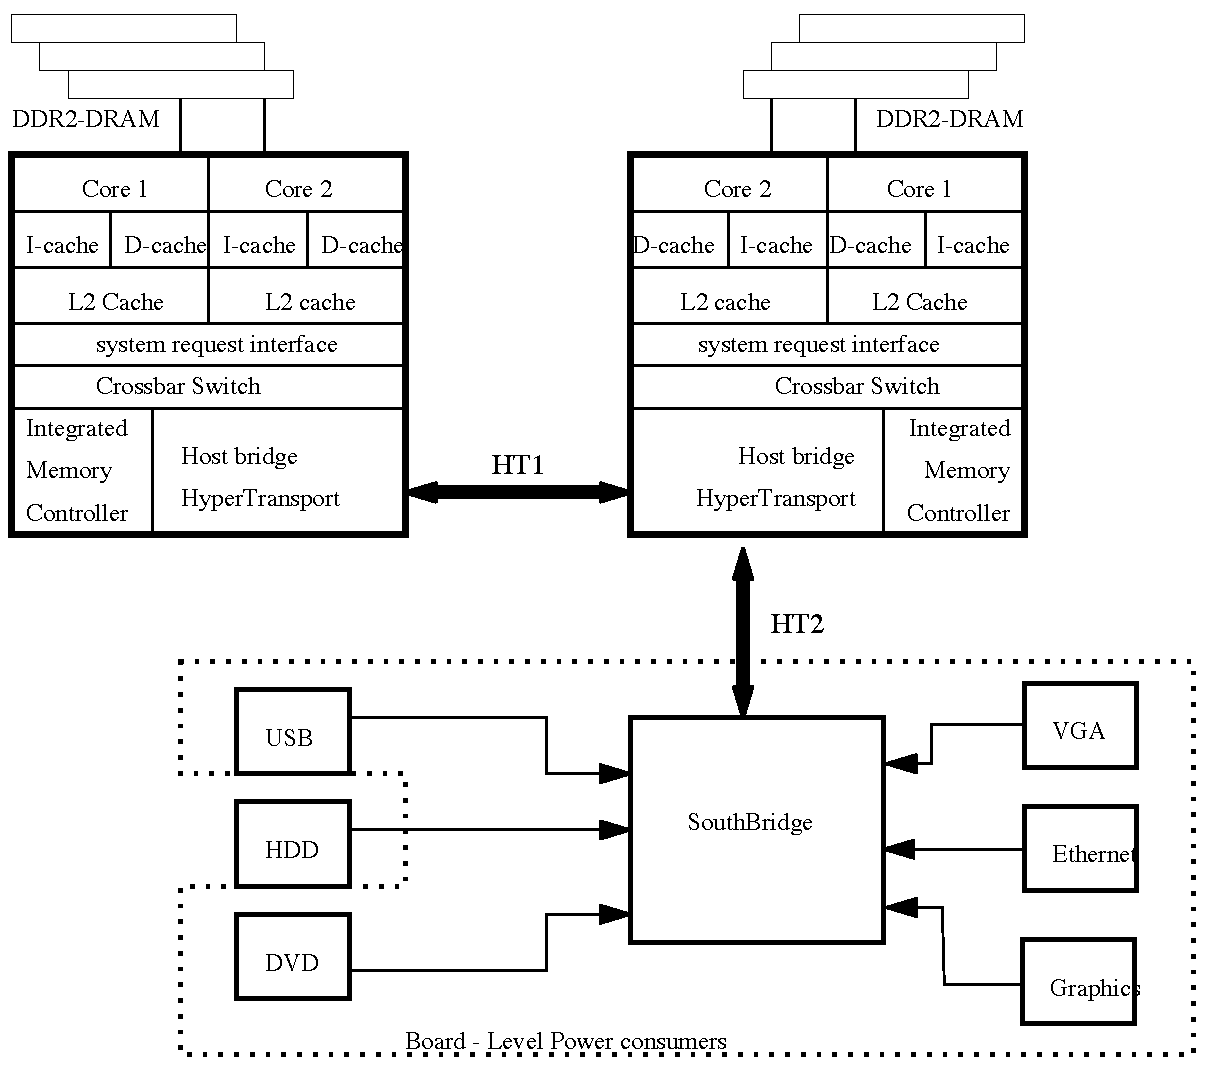
\includegraphics[scale=0.4]{x2200sys.pdf}
		\caption{Dual-core AMD Opteron based server architecture.}
		\label{fig:optarch}
	\end{center}
\end{figure}

Thus the total processor power consumption to reflect the thermal change due
to workload can be expressed as:
\begin{equation*}
\label{eqn:procpwr}
\bf{P_{proc}} =  \bf{H} \cdot \bf{X} 
 = [ \beta_0 \cdots \beta_{10} ]^T \cdot [ Var_0 \cdots Var_{10} ]^T
\end{equation*}
where $\bf{X}$ vector contains the following variables: ambient temperatures and
die temperatures for processors 0 and 1, HT1 and HT2 transactions, and
L2 cache misses per core.  The popularity of HyperTransport in server
and high performance computing platforms based on AMD, IBM, nVidia, Altera,
and Cray processors makes the model applicable to a wide
variety of platforms.
\subsection{DRAM energy}
\label{sec:dram}
Energy consumed by the DRAM banks can be computed by a combination of
measuring the counts of the highest level cache miss in the processor
combined with the DRAM Read/Write power along with the DRAM background
power(activation power).  As illustrated in \cite{Micron2007}, DRAM
background power and activation power can be obtained from the DRAM
datasheets.  For a single DRAM in our case, a total of 493mW would be
consumed. However, given the number of L2 cache misses per second when a
job is running on a certain core (over 22M / sec at the peak of bzip2
SPEC2006 benchmark), a significant amount of heat is generated from the
DRAM chips. The thermal airflow proximity of the DRAM banks to their
respective processors makes it possible for us to combine the energy
consumption and the consequent thermal output of the memory banks with the
processor ambient temperature. This value is reported by IPMI and we
combine it into our regression model.

\subsection{Hard disk energy}
\label{sec:networkengery}
The energy consumed by the hard disk while operating, can be
approximated to give an upper bound on the energy consumption of the
hard disk using a combination of performance counters and drive
ratings. In our server, Hitcahi's 7200 RPM 250G, SATA hard disk is
used. Table ~\ref{tab:hddparam} lists the typical power consumption
numbers for the hard disk used. Based on the physical, electrical and
electromechanical parameters of the hard disk, very detailed power
consumption models can be constructed. However we can achieve a cruder
but simpler model based on the typical power consumption data of the
hard disk and performance counters.

\begin{table*}
\centering
\caption{HItachi HDT725025VLA360 disk power parameters}
\begin{tabular}{ l l }
\hline
Parameter & Value \\
\hline
  Interface & Serial ATA  \\
  Capacity & 250 GB  \\
  Rotational speed & 7200 rpm  \\
  Power (spin up) & 5.25 W (max)  \\
  Power (Random read, write) & 9.4 W (typical)  \\
  Power (Silent read, write) & 7 W (typical)  \\
  Power (idle) & 5 W (typical)  \\
  Power (low RPM idle) & 2.3 W (typical for 4500 RPM)  \\
  Power (standby) & 0.8 W (typical)  \\
  Power (sleep) & 0.6 W (typical)  \\
\hline \hline
\end{tabular}
\label{tab:hddparam}
\end{table*}

The utility \texttt{iostat} can be used to measure the number of read
and writes per second to the disk as well as the kilobytes read from and
written to the disk. Thus based on this performance counter, we can
compute an approximate disk power consumption $E_{hdd}$ value as :
\begin{equation*}
\label{eqn:hddpwr1}
E_{hdd} = P_{spin-up}\times T_{su} 
        +  P_{read}\sum N_r\times T_r 
        + P_{write}\sum N_w\times T_w 
        + \sum P_{idle}\times T_{id}
\end{equation*}
where $P_{spin-up}$ is the power required to spin-up the disk from 0 to
full rotation. $T_{su}$ is the time required to achieve spin
up. $T_{su}$ is typically about 10s. $P_{read}$ is the power consumed
per kilobyte of data read from the disk. $N_r$ is the number of
kilobytes of data read in time-slice $T_r$ from the disk. The variables
are analogous for the write energy consumption. $P_{read}$ for our
Hitachi disk can be computed as follows:

The read operation at 1.5 Gbits/s consumes 530 mA current at +5V. Hence
every kilobyte read, consumes approximately $13.3 \mu
W$/Kbyte. Similarly, every write operation consumes $6.67 \mu
W$/Kbyte. The numbers $N_r$ and $N_w$ can be obtained using
\texttt{iostat} and out choice of time-slice.

The idle state has two conditions, idle and unloaded idle, where in the
latter case the heads are unloaded. The time to go from unloaded to idle
is usually less than 1 second, which is less than the resolution of
\texttt{iostat}. Thus, a history match count in the \texttt{iostat}
statistics where the reads and writes have been zero, tells us the
period in which the disk is idle, and the idle energy consumption can be
computed accordingly. \texttt{iostat} reading based conditions for
switching to different disk power states can be obtained with more
in-depth analysis, but the net results falls into this equation's
framework. That analysis is the topic of a future work.

The hard disk power can also be measured in real-time if current sensors
are provided at the output of the DC voltage lines delivering power to
the hard disk drives. The +5V lines will draw a maximum current of 730mA
and the +12V lines will draw a maximum current of 630mA. Thus $E_{hdd}$
can also be formulated as :
\begin{equation*}
\label{eq:hddpwr2}
E_{hdd} =  \int_{t1}^{t2} \left \{ v_1(t)\times i_1(t) + v_2(t)\times i_2(t) \right \} dt
\end{equation*}
This approach can be applied in the presence of current sensors which in
our experiments was measured with a current probe and logged through an
oscilloscope.

\subsection{Board Components}
\label{sec:board}
The quantity $E_{board}$ captures the energy required by the support
chipsets and usually fall in the 3.3V and 5V power
domains. In our case we obtain this value using current probe based
measurements. However, as in earlier cases, current
sensors for the power lines going into the board can provide
instantaneous energy draw from the power supply. The processor,
disk, fan, and optical-drive power lines are excluded here. For our
server, at most 28 additional current sensors might be required for
the entire blade \cite{SSI2004}. Thus:
\begin{equation*}
\label{eq:board}
E_{board} = \left(\sum V_{power-line}\times I_{power-line}\right) \times t_{time-slice}
\end{equation*}

\subsection{Electromechanical Energy}
\label{sec:electrical}
There is a basic electrical cost related to running the computer. The
quantity $E_{elect}$ in our model takes these quantities into account.
$E_{elect}$ is calculated as summation of the DC and AC power
consumption in the peripherals supporting the processor, particularly
the electromechanical components. This is mainly the power cosumption in
the power supply unit and the power consumption in the cooling fans.
As discussed earlier, the AC to DC conversion process is a load based number and
has a best case conversion efficiency of 80\% and a nominal efficiency of 75\% .

Power drawn by the fans for cooling can be given by the following equation:
\begin{equation*}
\label{eq:fanp}
P_{fan}=  P_{base} \cdot \left(\frac{RPM_{fan}}{RPM_{base}}\right)^3
\end{equation*} 
$P_{base}$ defines the base power consumption of the unloaded system. In our
case, that is the power consumption of the system when running only the
base operating system and no other jobs. That value is obtained
experimentally by measuring the current drawn on the +12V and +5V lines,
using a current probe and an oscilloscope. There is a current surge at
system startup, which is neglected and under nominal conditions, the
+12V line draws approximately 2.2A, which powers both the blowers fans
in the system. The two peripheral fans running at +5V draw around 2.1A
of current.  Thus the base power for the fans in known.  IPMI sensors
easily collect fan RPM data, and hence it is possible to quantify the
electrical power consumption in the system. Thus the electrical power
consumption can be quantified as:
\begin{equation*}
\label{eq:elect}
P_{elect}=  V(t) \cdot I(t) + \sum_{i=1}^NP_{i}
\end{equation*} 
where the first term in the equation is the instantaneous DC power
output from the power supply and is the DC power consumed by the
system. $N$ is the number of fans in the server and $P_{i}$ is the
instantaneous power consumed by the $i-th$ fan according to equation
~\ref{eq:fanp}. 
\begin{equation*}
\label{eq:elect}
\eta=  \frac{V(t) \cdot I(t)}{P_{in}}
\end{equation*} 
$\eta$ gives a measure of the energy conversion efficiency, into the
system from the mains, and gives an idea of the energy budget available
to the system.

Thus the total energy consumption during a given task period $T_{p}$ due
to electrical energy in the system can now be given by:
\begin{equation*}
\label{eq:elect}
E_{elect} =  \int^{T_{p}}_0 [V(t) \cdot I(t) + \sum_{i=1}^NP_{i}]\,dt
\end{equation*} 

\subsection{Combined Model}
\label{sec:wholemodel}

The total energy consumed by the system for a given computational
workload is modeled as a function of these metrics as:
\begin{equation*}
\label{eq:linmodel}
E_{system} =  \alpha_0 (E_{proc} + E_{mem}) + \alpha_1 E_{em} 
+ \alpha_2 E_{board} + \alpha_3 E_{hdd}
\end{equation*}
where $\alpha_{0}$,$\alpha_{1}$,$\alpha_{2}$, and $\alpha_{3}$ are unknown
constants that are determined through linear regression analysis and
remain constant for any given server architecture.

\section{Cache, Memory, Temperature, and Time}
\label{sec:timemodel}

We can rearrange the combined model in Equation~\ref{eq:linmodel} such
that we can solve the equations for the processor and memory energy
consumption:
\begin{align*}
  \alpha_0 (E_{proc} + E_{mem}) &= 
\end{align*}



\section{Experimental Study}
\label{sec:experiment}
\begin{table}
  \centering
  \caption{SPEC CPU2006 Benchmarks Used in Callibration}
  \label{tab:specbenchs}
  \begin{tabular}{c c l l}
    \hline
    Benchmark& &Type&Use\\
    \hline
    perlbench&C&Integer&PERL Programming Language\\
    bzip2&C&Integer&Compression\\
    mcf&C&Integer&Combinatorial Optimization\\
    omnetpp&C++&Integer&Discrete Event Simulation\\
    \hline
    gromacs&C/Fortran&Floating Point&Biochemistry/Molecular Dynamics\\
    cacstusADM&C/Fortran&Floating Point&Physics/General RElativity\\
    leslie3d&Fortran&Floating Point&Fluid Dynamics\\
    lbm&C&Floating Point&Fluid Dynamics\\
    \hline \hline
  \end{tabular}
\end{table}
\section{Application of Model to Physical System}
\label{sec:application}
The power model was calibrated to the system-under test (SUT) by
executing eight benchmarks from the SPEC CPU2006 benchmark suite
(Table~\ref{tab:specbenchs}). The benchmarks were selected using two
criteria: sufficient coverage of the functional units in the processor
and reasonable applicablity to the problem space.  Components of the
processor affect the thermal envelope in different
ways~\cite{Kumar2008}.  This issue is addressed by balancing the
benchmark selection between integer and floating point benchmarks in the
CPU2006 benchmark suite.  Second, the benchmarks were selected from the
suite based upon fit into the problem space.  Each benchmark represents
an application typical of the problems solved on high-performance
application servers.

\subsection{Hardware Environment}
\label{sec:hwenv}
\begin{table}
  \centering
  \label{tab:hardware}
  \caption{Test Hardware Configuration}
  \begin{tabular}{l|l}
    \hline
    &\textbf{Sun Fire 2200}\\  
    \hline 
    CPU&2 AMD Opteron\\
    CPU L2 cache&2x2MB\\
    Memory&8GB\\
    Internal disk&2060GB\\
    Network Interface Card&2x1000Mbps\\
    Video&On-board \\
    Height&1 rack unit\\
    \hline \hline
  \end{tabular}
\end{table}
The hardware used to evaluate our model is described in Table
\ref{tab:hardware}. The power consumed is measured with a WattsUP
\cite{WattsUp2006a} power meter connected between the AC Main and the
SUT.  The power meter measures the total and average wattage, voltage,
and amperage over the run of a workload.  The internal memory of the
power meter is cleared at the start of the run and the measures
collected during the run are downloaded after the run completes from the
meter's internal memory into a spreadsheet \cite{WattsUp2006b}.

Current flow on the different voltage domains in the server is measured
using an Agilent MSO6014A oscilloscope with one Agilent 1146A current
probe per system power domain (12v, 5v, and 3.3v). This data is
collected from the oscilloscope at the end of the execution of a
benchmark and stored in a spreadsheet on the test host.

\subsection{Software Environment}
\label{sec:software}
The operating system used in our setup is OpenSolaris (Solaris
11). System data is collected from the system baseboard controller using
the IPMI interface using the OpenSolaris \texttt{ipmitool} utility. Processor
performance counters are collected on a system-wide basis using the
OpenSolaris \texttt{cpustat} utility.

Five classes of metrics are sampled at 5 second intervals during the
experiment: (1) CPU temperature for all processors in the system, (2)
Ambient temperature in the computer case measured in one more locations
using the sensors provided by server manufacturer, (3) the number of
completed transactions processed through the system bus, and (4) the
number of misses that occur in the L2 cache associated with each CPU
core in the system.

\subsection{Discussion}
\label{sec:discussions}


\section{Conclusions and Future Work}
\label{sec:conclusions}

\label{sec:references}
\bibliographystyle{ULieeetran}

%\bibliography{cacheaffinity.bib}
\bibliography{../overall.bib}

\end{document}

